\documentclass{standalone}
\usepackage{tikz}
\usetikzlibrary{patterns, positioning}

\begin{document}
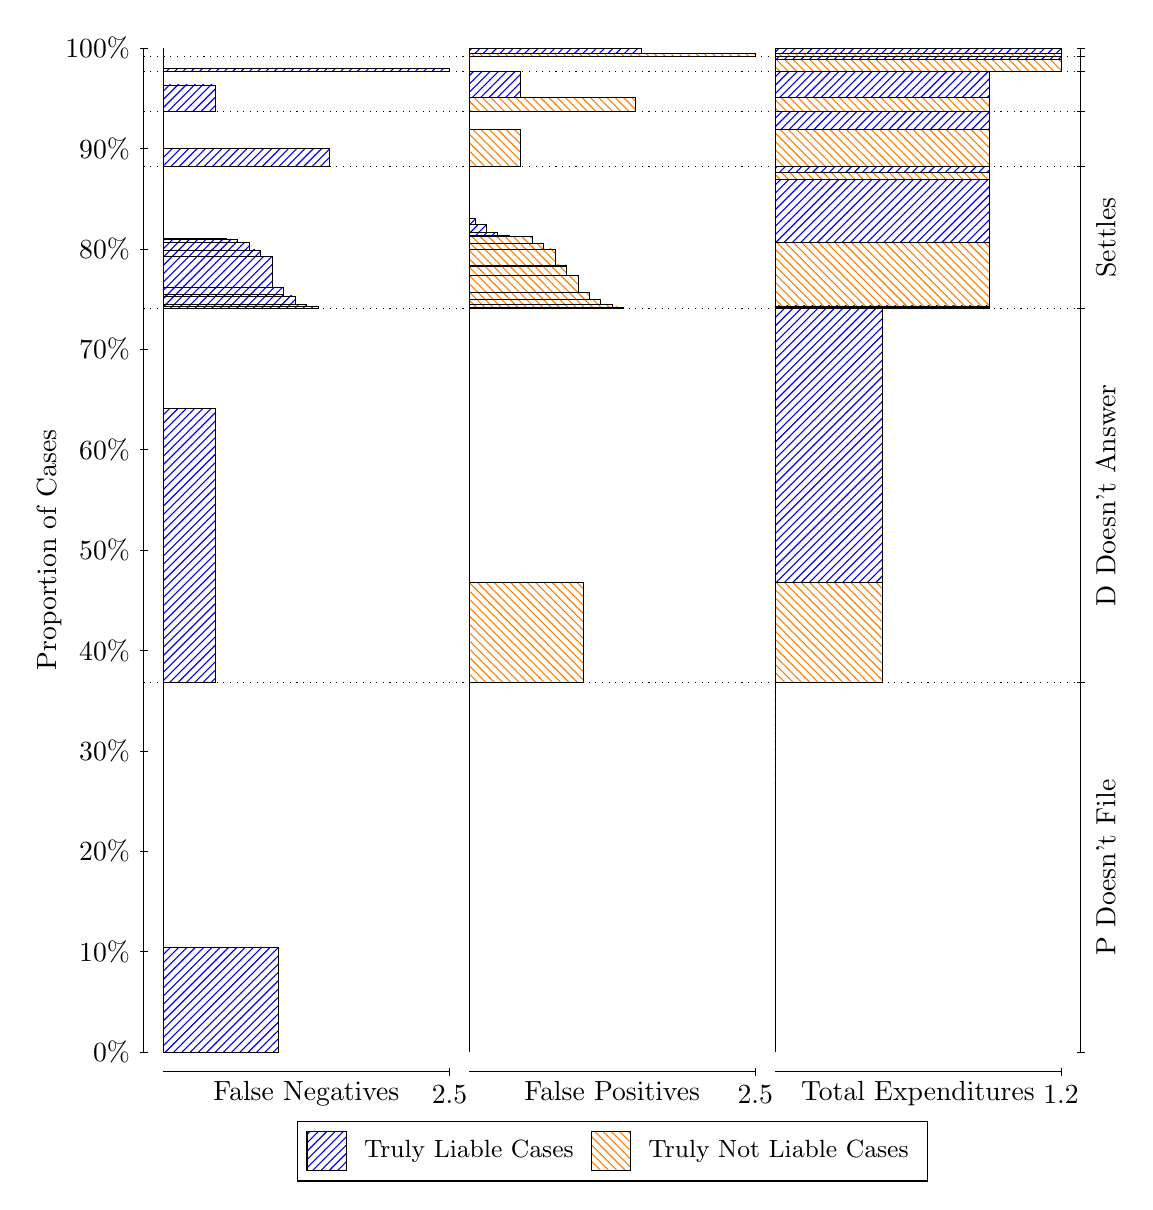
\begin{tikzpicture}
\draw[black, very thin] (1.5,1.75) -- (1.5,14.5);
\node[rotate=90, anchor=center] at (0.3, 8.125) {Proportion of Cases};
\draw[black, very thin] (1.45,1.75) -- (1.55,1.75);
\node[anchor=east] at (1.45, 1.75) {0\%};
\draw[black, very thin] (1.45,3.025) -- (1.55,3.025);
\node[anchor=east] at (1.45, 3.025) {10\%};
\draw[black, very thin] (1.45,4.3) -- (1.55,4.3);
\node[anchor=east] at (1.45, 4.3) {20\%};
\draw[black, very thin] (1.45,5.575) -- (1.55,5.575);
\node[anchor=east] at (1.45, 5.575) {30\%};
\draw[black, very thin] (1.45,6.85) -- (1.55,6.85);
\node[anchor=east] at (1.45, 6.85) {40\%};
\draw[black, very thin] (1.45,8.125) -- (1.55,8.125);
\node[anchor=east] at (1.45, 8.125) {50\%};
\draw[black, very thin] (1.45,9.4) -- (1.55,9.4);
\node[anchor=east] at (1.45, 9.4) {60\%};
\draw[black, very thin] (1.45,10.675) -- (1.55,10.675);
\node[anchor=east] at (1.45, 10.675) {70\%};
\draw[black, very thin] (1.45,11.95) -- (1.55,11.95);
\node[anchor=east] at (1.45, 11.95) {80\%};
\draw[black, very thin] (1.45,13.225) -- (1.55,13.225);
\node[anchor=east] at (1.45, 13.225) {90\%};
\draw[black, very thin] (1.45,14.5) -- (1.55,14.5);
\node[anchor=east] at (1.45, 14.5) {100\%};

\draw[black, very thin] (13.4,1.75) -- (13.4,14.5);
\draw[black, very thin] (13.35,1.75) -- (13.45,1.75);
\node[anchor=west] at (13.35, 1.75) {};
\draw[black, very thin] (13.35,6.442) -- (13.45,6.442);
\node[anchor=west] at (13.35, 6.442) {};
\draw[black, very thin] (13.35,11.195) -- (13.45,11.195);
\node[anchor=west] at (13.35, 11.195) {};
\draw[black, very thin] (13.35,12.998) -- (13.45,12.998);
\node[anchor=west] at (13.35, 12.998) {};
\draw[black, very thin] (13.35,13.698) -- (13.45,13.698);
\node[anchor=west] at (13.35, 13.698) {};
\draw[black, very thin] (13.35,14.202) -- (13.45,14.202);
\node[anchor=west] at (13.35, 14.202) {};
\draw[black, very thin] (13.35,14.392) -- (13.45,14.392);
\node[anchor=west] at (13.35, 14.392) {};
\draw[black, very thin] (13.35,14.5) -- (13.45,14.5);
\node[anchor=west] at (13.35, 14.5) {};

\draw[black, very thin, pattern color=blue, pattern=north east lines] (1.75,1.75) rectangle (3.2033,3.077);
\draw[black, very thin, pattern color=orange, pattern=north west lines] (1.75,3.077) rectangle (1.75,6.442);
\draw[black, very thin, pattern color=blue, pattern=north east lines] (1.75,6.442) rectangle (2.404,9.9264);
\draw[black, very thin, pattern color=orange, pattern=north west lines] (1.75,9.9264) rectangle (1.75,11.195);
\draw[black, very thin, pattern color=blue, pattern=north east lines] (1.75,11.195) rectangle (3.712,11.222);
\draw[black, very thin, pattern color=blue, pattern=north east lines] (1.75,11.222) rectangle (3.5667,11.246);
\draw[black, very thin, pattern color=blue, pattern=north east lines] (1.75,11.246) rectangle (3.4213,11.353);
\draw[black, very thin, pattern color=blue, pattern=north east lines] (1.75,11.353) rectangle (3.276,11.367);
\draw[black, very thin, pattern color=blue, pattern=north east lines] (1.75,11.367) rectangle (3.276,11.457);
\draw[black, very thin, pattern color=blue, pattern=north east lines] (1.75,11.457) rectangle (3.1307,11.857);
\draw[black, very thin, pattern color=blue, pattern=north east lines] (1.75,11.857) rectangle (2.9853,11.936);
\draw[black, very thin, pattern color=blue, pattern=north east lines] (1.75,11.936) rectangle (2.84,12.036);
\draw[black, very thin, pattern color=blue, pattern=north east lines] (1.75,12.036) rectangle (2.6947,12.074);
\draw[black, very thin, pattern color=blue, pattern=north east lines] (1.75,12.074) rectangle (2.5493,12.085);
\draw[black, very thin, pattern color=orange, pattern=north west lines] (1.75,12.085) rectangle (1.75,12.998);
\draw[black, very thin, pattern color=blue, pattern=north east lines] (1.75,12.998) rectangle (3.8573,13.23);
\draw[black, very thin, pattern color=orange, pattern=north west lines] (1.75,13.23) rectangle (1.75,13.698);
\draw[black, very thin, pattern color=blue, pattern=north east lines] (1.75,13.698) rectangle (2.404,14.031);
\draw[black, very thin, pattern color=orange, pattern=north west lines] (1.75,14.031) rectangle (1.75,14.202);
\draw[black, very thin, pattern color=blue, pattern=north east lines] (1.75,14.202) rectangle (5.3833,14.241);
\draw[black, very thin, pattern color=orange, pattern=north west lines] (1.75,14.241) rectangle (1.75,14.392);
\draw[black, very thin, pattern color=orange, pattern=north west lines] (1.75,14.392) rectangle (1.75,14.43);
\draw[black, very thin, pattern color=blue, pattern=north east lines] (1.75,14.43) rectangle (1.75,14.5);
\draw[black, very thin, pattern color=orange, pattern=north west lines] (5.6333,1.75) rectangle (5.6333,5.115);
\draw[black, very thin, pattern color=blue, pattern=north east lines] (5.6333,5.115) rectangle (5.6333,6.442);
\draw[black, very thin, pattern color=orange, pattern=north west lines] (5.6333,6.442) rectangle (7.0867,7.7108);
\draw[black, very thin, pattern color=blue, pattern=north east lines] (5.6333,7.7108) rectangle (5.6333,11.195);
\draw[black, very thin, pattern color=orange, pattern=north west lines] (5.6333,11.195) rectangle (7.5953,11.213);
\draw[black, very thin, pattern color=orange, pattern=north west lines] (5.6333,11.213) rectangle (7.45,11.242);
\draw[black, very thin, pattern color=orange, pattern=north west lines] (5.6333,11.242) rectangle (7.3047,11.31);
\draw[black, very thin, pattern color=orange, pattern=north west lines] (5.6333,11.31) rectangle (7.1593,11.393);
\draw[black, very thin, pattern color=orange, pattern=north west lines] (5.6333,11.393) rectangle (7.014,11.608);
\draw[black, very thin, pattern color=orange, pattern=north west lines] (5.6333,11.608) rectangle (6.8687,11.722);
\draw[black, very thin, pattern color=orange, pattern=north west lines] (5.6333,11.722) rectangle (6.8687,11.747);
\draw[black, very thin, pattern color=orange, pattern=north west lines] (5.6333,11.747) rectangle (6.7233,11.95);
\draw[black, very thin, pattern color=orange, pattern=north west lines] (5.6333,11.95) rectangle (6.578,12.023);
\draw[black, very thin, pattern color=orange, pattern=north west lines] (5.6333,12.023) rectangle (6.4327,12.108);
\draw[black, very thin, pattern color=blue, pattern=north east lines] (5.6333,12.108) rectangle (6.142,12.119);
\draw[black, very thin, pattern color=blue, pattern=north east lines] (5.6333,12.119) rectangle (5.9967,12.157);
\draw[black, very thin, pattern color=blue, pattern=north east lines] (5.6333,12.157) rectangle (5.8513,12.257);
\draw[black, very thin, pattern color=blue, pattern=north east lines] (5.6333,12.257) rectangle (5.706,12.336);
\draw[black, very thin, pattern color=blue, pattern=north east lines] (5.6333,12.336) rectangle (5.6333,12.998);
\draw[black, very thin, pattern color=orange, pattern=north west lines] (5.6333,12.998) rectangle (6.2873,13.466);
\draw[black, very thin, pattern color=blue, pattern=north east lines] (5.6333,13.466) rectangle (5.6333,13.698);
\draw[black, very thin, pattern color=orange, pattern=north west lines] (5.6333,13.698) rectangle (7.7407,13.869);
\draw[black, very thin, pattern color=blue, pattern=north east lines] (5.6333,13.869) rectangle (6.2873,14.202);
\draw[black, very thin, pattern color=orange, pattern=north west lines] (5.6333,14.202) rectangle (5.6333,14.353);
\draw[black, very thin, pattern color=blue, pattern=north east lines] (5.6333,14.353) rectangle (5.6333,14.392);
\draw[black, very thin, pattern color=orange, pattern=north west lines] (5.6333,14.392) rectangle (9.2667,14.43);
\draw[black, very thin, pattern color=blue, pattern=north east lines] (5.6333,14.43) rectangle (7.8133,14.5);
\draw[black, very thin, pattern color=orange, pattern=north west lines] (9.5167,1.75) rectangle (9.5167,5.115);
\draw[black, very thin, pattern color=blue, pattern=north east lines] (9.5167,5.115) rectangle (9.5167,6.442);
\draw[black, very thin, pattern color=orange, pattern=north west lines] (9.5167,6.442) rectangle (10.879,7.7108);
\draw[black, very thin, pattern color=blue, pattern=north east lines] (9.5167,7.7108) rectangle (10.879,11.195);
\draw[black, very thin, pattern color=orange, pattern=north west lines] (9.5167,11.195) rectangle (12.242,11.213);
\draw[black, very thin, pattern color=blue, pattern=north east lines] (9.5167,11.213) rectangle (12.242,11.225);
\draw[black, very thin, pattern color=orange, pattern=north west lines] (9.5167,11.225) rectangle (12.242,12.036);
\draw[black, very thin, pattern color=blue, pattern=north east lines] (9.5167,12.036) rectangle (12.242,12.835);
\draw[black, very thin, pattern color=orange, pattern=north west lines] (9.5167,12.835) rectangle (12.242,12.918);
\draw[black, very thin, pattern color=blue, pattern=north east lines] (9.5167,12.918) rectangle (12.242,12.998);
\draw[black, very thin, pattern color=orange, pattern=north west lines] (9.5167,12.998) rectangle (12.242,13.466);
\draw[black, very thin, pattern color=blue, pattern=north east lines] (9.5167,13.466) rectangle (12.242,13.698);
\draw[black, very thin, pattern color=orange, pattern=north west lines] (9.5167,13.698) rectangle (12.242,13.869);
\draw[black, very thin, pattern color=blue, pattern=north east lines] (9.5167,13.869) rectangle (12.242,14.202);
\draw[black, very thin, pattern color=orange, pattern=north west lines] (9.5167,14.202) rectangle (13.15,14.353);
\draw[black, very thin, pattern color=blue, pattern=north east lines] (9.5167,14.353) rectangle (13.15,14.392);
\draw[black, very thin, pattern color=orange, pattern=north west lines] (9.5167,14.392) rectangle (13.15,14.43);
\draw[black, very thin, pattern color=blue, pattern=north east lines] (9.5167,14.43) rectangle (13.15,14.5);
\draw[black, dotted] (1.5,6.442) -- (13.4,6.442);
\draw[black, dotted] (1.5,11.195) -- (13.4,11.195);
\draw[black, dotted] (1.5,12.998) -- (13.4,12.998);
\draw[black, dotted] (1.5,13.698) -- (13.4,13.698);
\draw[black, dotted] (1.5,14.202) -- (13.4,14.202);
\draw[black, dotted] (1.5,14.392) -- (13.4,14.392);
\draw[black, very thin] (1.75,1.5) -- (5.3833,1.5);
\node[anchor=north] at (3.5667, 1.5) {False Negatives};
\draw[black, very thin] (5.3833,1.45) -- (5.3833,1.55);
\node[anchor=north] at (5.3833, 1.45) {2.5};

\draw[black, very thin] (5.6333,1.5) -- (9.2667,1.5);
\node[anchor=north] at (7.45, 1.5) {False Positives};
\draw[black, very thin] (9.2667,1.45) -- (9.2667,1.55);
\node[anchor=north] at (9.2667, 1.45) {2.5};

\draw[black, very thin] (9.5167,1.5) -- (13.15,1.5);
\node[anchor=north] at (11.333, 1.5) {Total Expenditures};
\draw[black, very thin] (13.15,1.45) -- (13.15,1.55);
\node[anchor=north] at (13.15, 1.45) {1.2};

\node[black, centered, rotate=90] at (13.72, 4.096) {P Doesn't File};
\node[black, centered, rotate=90] at (13.72, 8.8186) {D Doesn't Answer};
\node[black, centered, rotate=90] at (13.72, 12.096) {Settles};





\draw (7.449999999999999,1.5) node[draw=none] (baseCoordinate) {};
\begin{scope}[align=center]
        \matrix[scale=0.5, draw=black, below=0.5cm of baseCoordinate, nodes={draw}, column sep=0.1cm]{
            \node[rectangle, draw, minimum width=0.5cm, minimum height=0.5cm, pattern=north east lines, pattern color=blue] {}; &
            \node[draw=none, font=\small] (B) {Truly Liable Cases}; &
            \node[rectangle, draw, minimum width=0.5cm, minimum height=0.5cm, pattern=north west lines, pattern color=orange] {}; &
            \node[draw=none, font=\small] (B) {Truly Not Liable Cases}; \\
            };
\end{scope}

\end{tikzpicture}
\end{document}